\section{Workflows Implemented in BiobankCloud}
Next generation sequencing, a technology first introduced to the market in 2005, has revolutionized biological research during the last ten years~\cite{shendure2008next}. This technology allows scientist to study not only the genome of any species, but also the transcriptome and the epigenome.
We have implemented several pipelines for the analysis of the most common types of next generation sequencing data into the BiobankCloud. 

\textbf{Variant Calling pipeline:} Genetic variations represent changes in the order of the bases in a DNA sequence and variations in the human genome play a decisive role in human disease. The most common variations in the genome are the single nucleotide variations and short insertions and deletions. For this pipeline, whole genome sequencing and/or whole exome sequencing data can be chosen as input data and the workflow was derived from Thalheim \cite{snp_wf_thalheim}. Figure \ref{fig:workflow_snp} shows a schematic overview on this Variant Calling pipeline built in BiobankCloud.


\vskip-5pt
\begin{figure}[h]
\centering
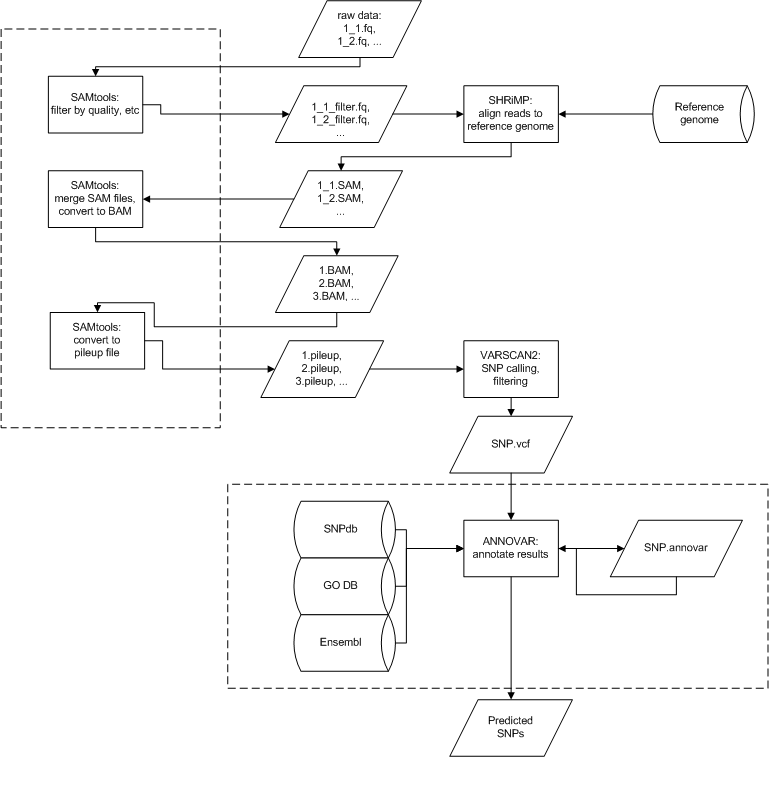
\includegraphics[width=0.6\textwidth]{./imgs/wf_snp.png}
\caption{Subsequent processing steps in BiobankCloud's Variant Calling pipeline.}
\label{fig:workflow_snp}
\end{figure}
\vskip-5pt


\textbf{Gene Expression pipeline:} This pipeline uses RNA-Seq data as input and enables the user to study differential expression on different levels such as 
genes and transcripts. Furthermore, it detects differential splicing and promoter use between two or more groups of interest.
The pipeline was implemented according to Trapnell et al.\cite{trapnell2012differential, trapnell2013differential}.

\textbf{ChIP-Seq pipeline:} ChIP-Seq (Chromatin immunoprecipitation coupled with high-throughput sequencing) is the standard technique for studying the genome-wide binding profiles of DNA-binding proteins, e.g. transcription factors, as well as the distribution of histone modifications. ChIP-Seq NGS data are the input data for this pipeline and the workflow is described by Dimitrova et al. \cite{dimitrova2014pax5} was used.

\textbf{microRNA pipeline:} microRNAs are short expressed RNAs that play a key role in many biological processes and in different diseases. Our pipeline for analysis of the expression profiles of microRNAs is based on the publication of Kozubek et al. \cite{kozubek2013depth} and is using small RNA-Seq data as input.




